\documentclass[10pt]{beamer}

\usetheme{metropolis}
\usepackage{appendixnumberbeamer}

\usepackage{booktabs}
\usepackage[scale=2]{ccicons}

\usepackage{pgfplots}
\usepgfplotslibrary{dateplot}

\usepackage{xspace}
\newcommand{\themename}{\textbf{\textsc{metropolis}}\xspace}

\usepackage{ltablex} % Tables
\usepackage{ragged2e} % Text Alignment in Tables

\title{Model Transformations for DSL Processing}
\date{January 14, 2019}
\author{Stefan Kapferer}
\institute{University of Applied Sciences of Eastern Switzerland (HSR FHO)}
% \titlegraphic{\hfill\includegraphics[height=1.5cm]{logo.pdf}}

\usepackage{url}
\def\UrlNoBreaks{\do\:}

\usepackage{amsmath}

\usepackage{listings,lstautogobble}
\usepackage{minted}
\usemintedstyle{vs}

\usepackage{mathtools}

\usepackage[absolute,overlay]{textpos}
  \setlength{\TPHorizModule}{1mm}
  \setlength{\TPVertModule}{1mm}

\graphicspath{ {./images/} }

\begin{document}

\maketitle

\begin{frame}{Table of contents}
  \setbeamertemplate{section in toc}[sections numbered]
  \tableofcontents[hideallsubsections]
\end{frame}

\section{Introduction: Model Transformation}

\begin{frame}[fragile]{Models}

	Models are used in \textbf{all disciplines and phases} of the \textbf{software development lifecycle}:
	\begin{itemize}
  		\item \textbf{Business Modeling}: Domain Models, Use Case Models, ...
  		\item \textbf{Analysis \& Design}: Architecture View Models, Context Maps ...
  		\item \textbf{Implementation}: Class Models, Object Models, Data Models, ...
  		\item \textbf{Testing}: Performance Simulation Models, ...
  		\item \textbf{Operations \& Maintenance}: Deployment Models, ...
  	\end{itemize}

\end{frame}

\begin{frame}[fragile]{Model Transformation}

	\textbf{Goal:} Transform a model into another model.	
	\bigskip
	
	\textbf{Models differ in:}
	\begin{itemize}
		\item Level of abstraction
		\item Representation / Language
		\item Metamodel (Eclipse Ecore, UML, ...)
	\end{itemize}
		
	\bigskip
	\textbf{Examples:}
	\begin{itemize}
		\item Change level of abstraction
		\begin{itemize}
			\item Refinement of domain model towards fully-fledged class diagram
		\end{itemize}
		\item Change representation or language (keep semantics)
		\begin{itemize}
			\item Refactorings
			\item Code migration into other language
		\end{itemize}
	\end{itemize}

\end{frame}

% \begin{frame}[fragile]{Model Transformation Taxonomy \cite{MENS2006125}}

% Different types of model transformations:

% \begin{itemize}
% 	\item \textbf{Endogenous vs. Exogenous}
% 	\begin{itemize}
% 		\item Endogenous: Source and target model are represented by the same language
% 		\item Exogenous: Transformation between models in different languages/representations
% 	\end{itemize}
% 	\item \textbf{In-place vs. Out-place}
% 	\begin{itemize}
% 		\item Concerns endogenous transformations only. Exogenous transformations are always out-place.
% 		\item In-place: Transformation within the same meta-model
% 		\item Out-place: Source meta-model differs from output meta-model
% 	\end{itemize}
% 	\item \textbf{Horizontal vs. Vertical}
% 	\begin{itemize}
% 		\item Horizontal: Source and target model are on same level of abstraction
% 		\item Vertical: Transformation changes the level of abstraction
% 	\end{itemize}
% \end{itemize}

% \end{frame}

\section{DSL Example \& Live Demo}

\begin{frame}{ContextMapper DSL \cite{contextmapper}}
	\textbf{A Domain-specific Language for Context Mapping \linebreak \& Service Decomposition}\footnote{\url{https://contextmapper.github.io/}}
	
	\begin{textblock}{20}(92,15)
		\includegraphics[scale=0.3]{./images/cm-logo-github.png}
    \end{textblock}	
	
	\begin{itemize}
		\item Modeling Domain-driven Design (DDD) Context Maps
		\item Goal: Apply model transformations to realize architectural refactorings \cite{ZimmermannArchitecturalRefactorings} towards service decomposition
		\begin{itemize}
			\item Split bounded contexts
		\end{itemize}
	\end{itemize}
	
	\textbf{DSL Processing via Model Transformation}:
	\begin{itemize}
		\item DSL Text $\xrightarrow{parsing}$ Abstract Syntax Tree (AST) $\xrightarrow{}$ Model
		\item Model $\xrightarrow{transformation}$ Model
		\item Model $\xrightarrow{}$ Abstract Syntax Tree (AST) $\xrightarrow{unparsing}$ DSL Text
	\end{itemize}
\end{frame}

\begin{frame}[fragile]{ContextMapper DSL Example Context Map}
	\textbf{Example Context Map:}
	
\begin{minted}[frame=single,linenos,fontsize=\scriptsize]{cml-lexer.py:CMLLexer -x}
ContextMap {
  /* Add Bounded Contexts to Context Map */
  contains CustomerManagement
  contains CustomerSelfService
  contains PolicyManagement
  contains DebtCollection
  
  /* Define Bounded Context Relationships: */
  
  CustomerSelfService -> CustomerManagement : Customer-Supplier
  
  PolicyManagement -> CustomerManagement : Upstream-Downstream {
    implementationTechnology = "RESTful HTTP"
    upstream implements OPEN_HOST_SERVICE, PUBLISHED_LANGUAGE
    downstream implements CONFORMIST
  }
  
  PolicyManagement <-> DebtCollection : Shared-Kernel {
    implementationTechnology = "Shared Java Library"
  }
}
\end{minted}

\end{frame}

\begin{frame}[fragile]{ContextMapper DSL Example: Input}
	\textbf{DSL snippet modeling a bounded context:}
	
\begin{minted}[frame=single,linenos,fontsize=\scriptsize]{cml-lexer.py:CMLLexer -x}
/* Example Bounded Context in CML */
BoundedContext CustomerManagement {
  Aggregate Customers {
    Entity Customer {
      String firstName
      String familyName
      Account customerBankAccount
    }
    Entity Account {
      String iban
      String bankName
    }
  } 
  Aggregate CustomerSelfService {
    Entity Account {
      String username
      String password
      Customer owner
    }
  }
}
\end{minted}

\end{frame}

\begin{frame}[standout]
  Live Demo: «Split Bounded Context by Duplicate Entity Name»
\end{frame}

\begin{frame}[fragile]{ContextMapper DSL Example: Output}
\begin{minted}[frame=single,linenos,fontsize=\scriptsize]{cml-lexer.py:CMLLexer -x}
/* Example Bounded Context in CML */
BoundedContext CustomerManagement {
  Aggregate Customers {
    Entity Customer{
      String firstName
      String familyName
      Account customerBankAccount
    }
    Entity Account {
      String iban
      String bankName
    }
  } 
}
BoundedContext SplitBoundedContext {
  Aggregate CustomerSelfService {
    Entity Account {
      String username
      String password
      Customer owner
    }
  }
}
\end{minted}

\end{frame}


\section{Model Transformations with Henshin}

\begin{frame}{Henshin Transformation Tool}
	\textbf{Henshin \cite{Arendt:2010:HAC:1926458.1926471}} is an EMF \cite{steinberg2008emf} based transformation tool.
	
	\begin{textblock}{20}(92,15)
		\includegraphics[scale=1.0]{./images/henshin_logo.png}
    \end{textblock}		
	
	\begin{itemize}
		\item \textit{Henshin} means transformation in Japanese
		\item Supports in-place model transformations
		\item Endogenous \& Exogenous
		\item Horizontal \& Vertical
	\end{itemize}
	
	\begin{itemize}
		\item Based on Algebraic Graph Transformation \cite{DBLP:series/eatcs/EhrigEPT06}
	\end{itemize}
\end{frame}

\begin{frame}{The Henshin Transformation Meta-Model\footnote{Copied from \url{https://wiki.eclipse.org/Henshin/Transformation\_Meta-Model}}}
	\begin{figure}[H]
		\centering
		\includegraphics[width=1.0\textwidth]{Henshin_Transformation_Modules}
	\end{figure} 
\end{frame}

\begin{frame}{Example Transformation Model}
	\textbf{Transformation model for example seen in the live demo:}
	\begin{itemize}
		\item LHS graph: «preserve» $+$ «delete»
		\item RHS graph: «preserve» $+$ «create»
	\end{itemize}
	\begin{figure}[H]
		\centering
		\includegraphics[width=1.0\textwidth]{ContextMapRefactoring_Example}
	\end{figure} 
\end{frame}

\section{Algebraic Graph Transformation}

\begin{frame}[fragile]{From String Grammars ...}

\textbf{The classical string grammar you know:}

\begin{center}
\begin{lstlisting}
DecimalNumeral -> 0 | NonZeroDigit Digits
Digits         -> ε | Digit | Digits Digit
Digit          -> 0 | NonZeroDigit
NonZeroDigit   -> 1 | 2 | 3 | 4 | 5 | 6 | 7 | 8 | 9
\end{lstlisting}
\end{center}

\begin{itemize}
	\item Example: \textit{DecimalNumeral} grammar of the Java Language Specification in Backus-Naur Form (BNF).
	\item String grammar consists of a \textbf{set of production rules}.
\end{itemize}

\end{frame}

\begin{frame}{... to Graph Grammars}

	\textbf{Similar principle with graphs:}

	\begin{itemize}
		\item Left-hand side (LHS) of the rule has to be matched in graph on which the rule is applied to.
		\item Right-hand side (RHS) describes the changes which will be applied
	\end{itemize}

	\begin{figure}[H]
		\centering
		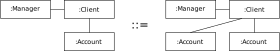
\includegraphics[width=0.8\textwidth]{grammar_rule_example}
	\end{figure} 
	
	\textbf{Example:} Banking scenario «create new account for a customer».

\end{frame}

\begin{frame}{Pushout Operation}

The so-called \textbf{pushout} is an operator transforming a graph $G$ into another graph $G'$ given a production $p$ (graph grammar rule) and two graph morphisms.

\begin{figure}[H]
	\centering
	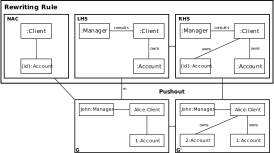
\includegraphics[width=1.0\textwidth]{banking-example-pushout}
\end{figure} 

\end{frame}

\section{Summary \& Conclusions}

\begin{frame}{Seminar Question \#1: \\Model Transformation vs. Program Transformation}

	\begin{itemize}
		\item Other \textbf{software engineering disciplines}
		\begin{itemize}
			\item Business Modeling, Analysis \& Design vs. Implementation
		\end{itemize}
		\item Other \textbf{level of abstraction}
	\end{itemize}
	
	\begin{itemize}
		\item \textbf{Model Transformations}
		\begin{itemize}
			\item model-to-model
			\item model-to-code
			\item code-to-model
		\end{itemize}
		\item \textbf{Program Transformations}
		\begin{itemize}
			\item code-to-code
		\end{itemize}
	\end{itemize}
	
	\textbf{Note:} Refactoring (code-to-code) can be implemented as model transformation too.

\end{frame}

\begin{frame}{Seminar Question \#2: \\Henshin Maturity \& Differences to other Tools}

	\begin{itemize}
		\item Henshin \textbf{Conclusion}:
		\begin{itemize}
			\item + Expressive transformation specification
	  		\item + Mature transformation engine
  			\item + Solid foundations
  			\item - Improvable Tooling
		\end{itemize}
	\end{itemize}
	
	\begin{itemize}
		\item Main \textbf{differences} to other transformation approaches:
		\begin{itemize}
			\item Not only theoretic research project
			\begin{itemize}
				\item Good compromise between scientific foundations \& feasible tool implementation
			\end{itemize}
			\item Declarative transformation specification
			\begin{itemize}
				\item Other tools often use imperative approaches
			\end{itemize}
		\end{itemize}
	\end{itemize}

\end{frame}

\begin{frame}{Seminar Question \#3: \\Model Transformation for DSL Processing}

	\begin{itemize}
		\item DSL as a customized \textbf{model representation}
		\item DSL text can be transformed into other model representations
		\item Example:
		\begin{itemize}
			\item DSL to EMF model («\textbf{Parsing}»)
			\item EMF model to DSL («\textbf{Unparsing}»)
		\end{itemize}
	\end{itemize}
	\bigskip
	\begin{itemize}
		\item \textbf{DSL processing} approach:
		\begin{itemize}
			\item DSL Text $\xrightarrow{parsing}$ Abstract Syntax Tree (AST) $\xrightarrow{}$ Model
			\item Model $\xrightarrow{transformation}$ Model
			\item Model $\xrightarrow{}$ Abstract Syntax Tree (AST) $\xrightarrow{unparsing}$ DSL Text
		\end{itemize}
	\end{itemize}

\end{frame}

\section{Questions \& Discussion}

\begin{frame}[standout]
  Questions?
\end{frame}

\begin{frame}[standout]
  Discussion
\end{frame}

\appendix

\begin{frame}[allowframebreaks]{References}

  \bibliography{presentation}
  \bibliographystyle{abbrv}

\end{frame}

\end{document}
